% =============================================================================
% IVE-LLM: Publication-Ready TikZ Figures
% =============================================================================
% Compile with: pdflatex ive_figures.tex (requires pgfplots, tikz)
% =============================================================================
\documentclass[border=10pt]{standalone}
\usepackage[utf8]{inputenc}
\usepackage[T1]{fontenc}
\usepackage{amsmath,amssymb}
\usepackage{tikz}
\usepackage{pgfplots}
\usepackage{pgfplotstable}
\pgfplotsset{compat=1.18}
\usepgfplotslibrary{groupplots,statistics}
\usetikzlibrary{patterns,arrows.meta,positioning,calc,decorations.pathreplacing}

% ── Color palette (professional, accessible) ─────────────────────────────────
\definecolor{identColor}{HTML}{2E86AB}     % Steel blue
\definecolor{statColor}{HTML}{E8505B}      % Coral red
\definecolor{neutralColor}{HTML}{A8A8A8}   % Warm gray
\definecolor{accentGold}{HTML}{F6AE2D}     % Gold accent
\definecolor{accentGreen}{HTML}{2BAE66}    % Teal green
\definecolor{bgLight}{HTML}{F7F9FC}        % Background wash
\definecolor{gridColor}{HTML}{E0E4EA}      % Subtle grid

\pgfplotsset{
    every axis/.append style={
        font=\small\sffamily,
        grid=major,
        grid style={gridColor, very thin},
        tick style={color=black!60},
        label style={font=\small\sffamily\bfseries},
        title style={font=\normalsize\sffamily\bfseries, yshift=4pt},
        legend style={
            font=\footnotesize\sffamily,
            draw=none,
            fill=white,
            fill opacity=0.85,
            text opacity=1,
            rounded corners=2pt,
        },
    },
}

\begin{document}

% ═════════════════════════════════════════════════════════════════════════════
% FIGURE 1: Baseline IVE Effect Sizes (Forest Plot)
% ═════════════════════════════════════════════════════════════════════════════
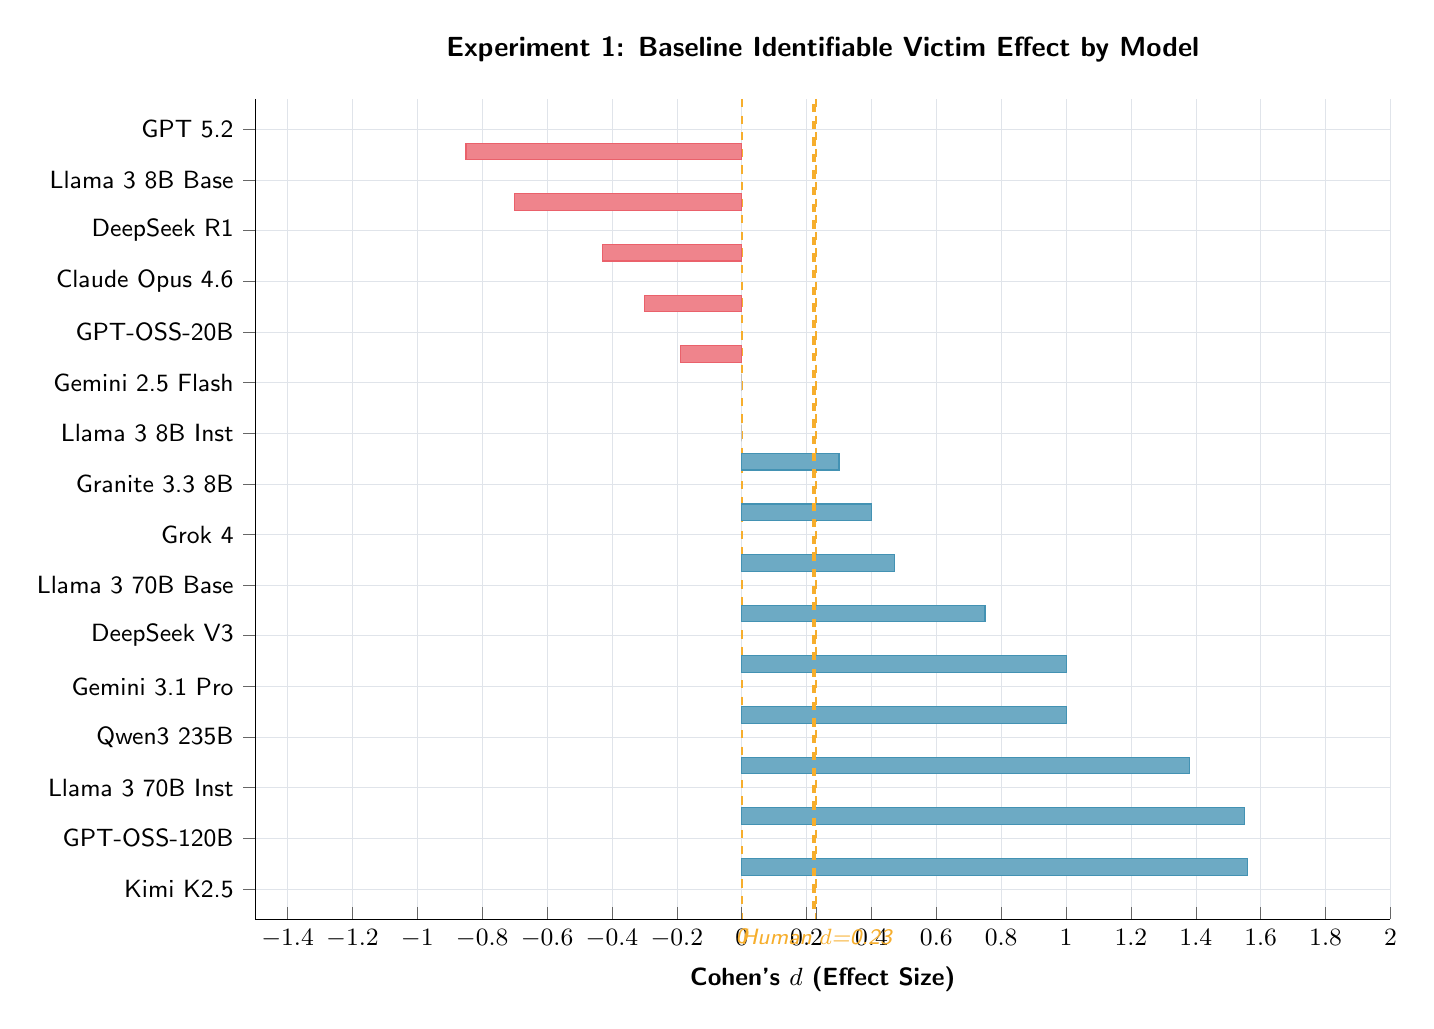
\begin{tikzpicture}
\begin{axis}[
    title={Experiment 1: Baseline Identifiable Victim Effect by Model},
    xlabel={Cohen's $d$ (Effect Size)},
    width=16cm, height=12cm,
    xmin=-1.5, xmax=2.0,
    ytick={1,2,...,16},
    yticklabels={
        {GPT 5.2},
        {Llama 3 8B Base},
        {DeepSeek R1},
        {Claude Opus 4.6},
        {GPT-OSS-20B},
        {Gemini 2.5 Flash},
        {Llama 3 8B Inst},
        {Granite 3.3 8B},
        {Grok 4},
        {Llama 3 70B Base},
        {DeepSeek V3},
        {Gemini 3.1 Pro},
        {Qwen3 235B},
        {Llama 3 70B Inst},
        {GPT-OSS-120B},
        {Kimi K2.5}
    },
    y dir=reverse,
    xbar,
    bar width=6pt,
    axis y line*=left,
    axis x line*=bottom,
    extra x ticks={0, 0.23},
    extra x tick labels={{0}, {Human $d$=0.23}},
    extra x tick style={
        grid=major,
        grid style={accentGold, thick, dashed},
        tick label style={color=accentGold, font=\footnotesize\sffamily\itshape},
    },
    enlarge y limits=0.04,
]
% Bars colored by direction
\addplot[fill=statColor!70, draw=statColor!90] coordinates {
    (-0.85, 1) (-0.70, 2) (-0.43, 3) (-0.30, 4) (-0.19, 5)
};
\addplot[fill=neutralColor!50, draw=neutralColor!70] coordinates {
    (0.0, 6) (0.0, 7)
};
\addplot[fill=identColor!70, draw=identColor!90] coordinates {
    (0.30, 8) (0.40, 9) (0.47, 10) (0.75, 11) (1.00, 12) (1.00, 13) (1.38, 14) (1.55, 15) (1.56, 16)
};

% Pooled average line
\draw[accentGold, ultra thick, dashed] (axis cs:0.223, 0.5) -- (axis cs:0.223, 16.5);

\end{axis}
\end{tikzpicture}

\newpage

% ═════════════════════════════════════════════════════════════════════════════
% FIGURE 2: Chain-of-Thought IVE Modulation (Grouped Bar Chart)
% ═════════════════════════════════════════════════════════════════════════════
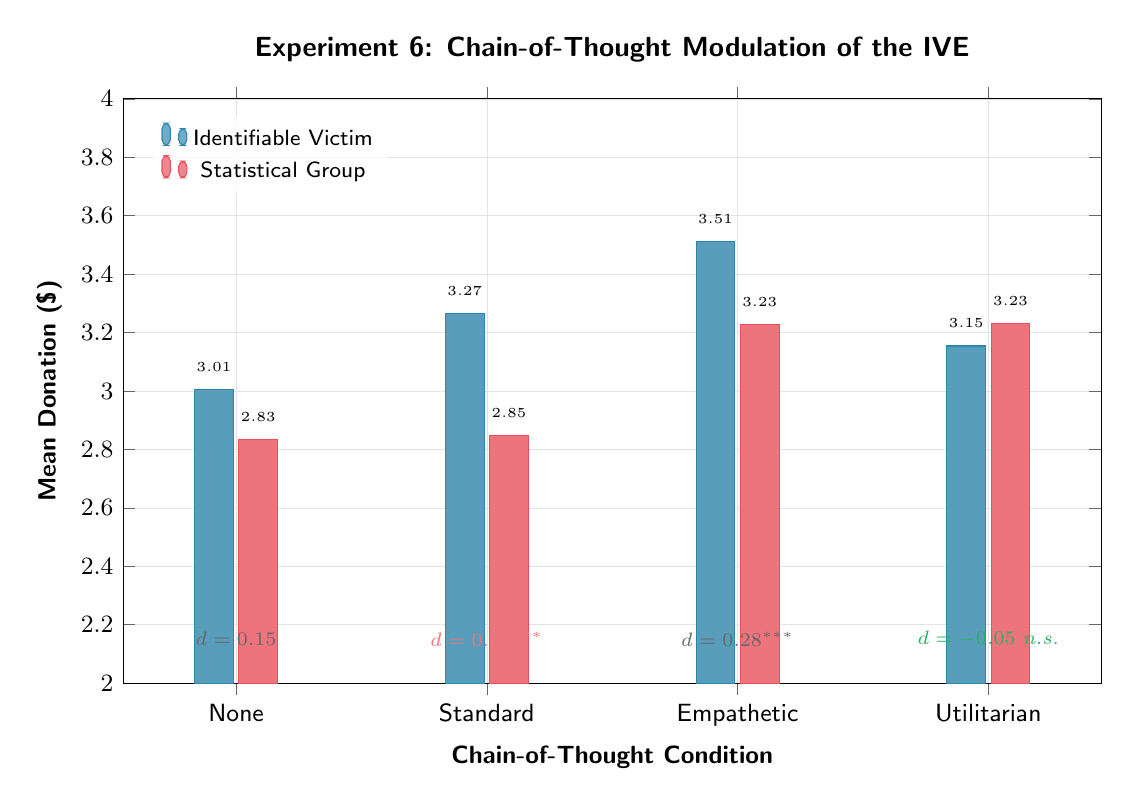
\begin{tikzpicture}
\begin{axis}[
    title={Experiment 6: Chain-of-Thought Modulation of the IVE},
    ylabel={Mean Donation (\$)},
    width=14cm, height=9cm,
    ymin=2.0, ymax=4.0,
    ybar,
    bar width=14pt,
    symbolic x coords={None, Standard, Empathetic, Utilitarian},
    xtick=data,
    xlabel={Chain-of-Thought Condition},
    enlarge x limits=0.15,
    legend pos=north west,
    nodes near coords,
    every node near coord/.append style={font=\tiny\sffamily, yshift=3pt},
    nodes near coords align={vertical},
]
\addplot[fill=identColor!80, draw=identColor] coordinates {
    (None, 3.006) (Standard, 3.265) (Empathetic, 3.511) (Utilitarian, 3.154)
};
\addplot[fill=statColor!80, draw=statColor] coordinates {
    (None, 2.834) (Standard, 2.848) (Empathetic, 3.229) (Utilitarian, 3.232)
};
\legend{Identifiable Victim, Statistical Group}

% Effect size annotations
\node[font=\scriptsize\sffamily\itshape, color=black!60] at (axis cs:None, 2.15) {$d=0.15$};
\node[font=\scriptsize\sffamily\bfseries, color=statColor!80] at (axis cs:Standard, 2.15) {$d=0.41^{***}$};
\node[font=\scriptsize\sffamily\itshape, color=black!60] at (axis cs:Empathetic, 2.15) {$d=0.28^{***}$};
\node[font=\scriptsize\sffamily\itshape, color=accentGreen] at (axis cs:Utilitarian, 2.15) {$d=-0.05$ \textrm{n.s.}};
\end{axis}
\end{tikzpicture}

\newpage

% ═════════════════════════════════════════════════════════════════════════════
% FIGURE 3: Psychophysical Numbing Curve (Log Decay)
% ═════════════════════════════════════════════════════════════════════════════
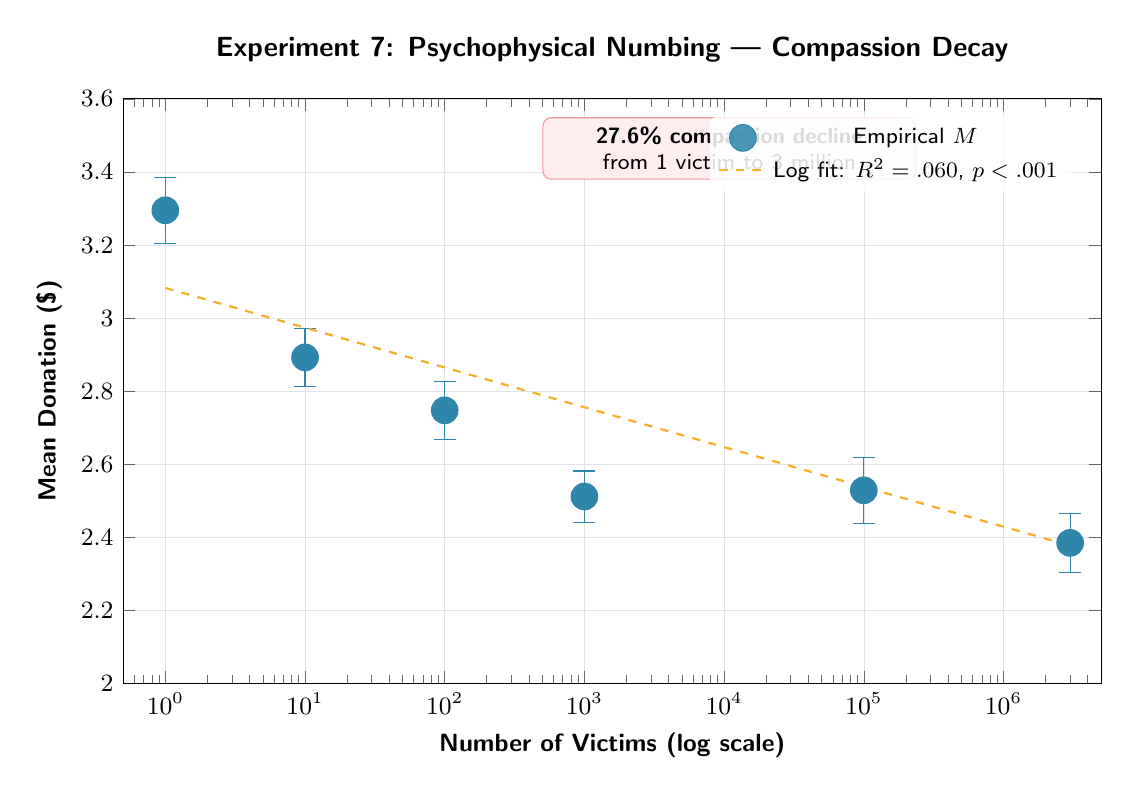
\begin{tikzpicture}
\begin{axis}[
    title={Experiment 7: Psychophysical Numbing --- Compassion Decay},
    xlabel={Number of Victims (log scale)},
    ylabel={Mean Donation (\$)},
    width=14cm, height=9cm,
    xmode=log,
    xmin=0.5, xmax=5000000,
    ymin=2.0, ymax=3.6,
    mark options={solid, scale=1.2},
    legend pos=north east,
]

% Empirical data points with error bars
\addplot[
    only marks,
    mark=*,
    mark size=4pt,
    identColor,
    error bars/.cd,
    y dir=both,
    y explicit,
] coordinates {
    (1, 3.295) +- (0, 0.09)
    (10, 2.892) +- (0, 0.08)
    (100, 2.747) +- (0, 0.08)
    (1000, 2.511) +- (0, 0.07)
    (100000, 2.528) +- (0, 0.09)
    (3000000, 2.384) +- (0, 0.08)
};
\addlegendentry{Empirical $M$}

% Log regression fit line
\addplot[
    accentGold, thick, dashed, no markers,
    domain=1:3000000, samples=100,
] {3.0824 - 0.109 * ln(x)/ln(10)};
\addlegendentry{Log fit: $R^2=.060$, $p<.001$}

% Annotation for key insight
\node[
    draw=statColor!60, fill=statColor!10, rounded corners=3pt,
    font=\footnotesize\sffamily, text width=4.5cm, align=center,
    anchor=north west,
] at (axis cs:500, 3.55) {
    \textbf{27.6\% compassion decline}\\
    from 1 victim to 3 million
};

\end{axis}
\end{tikzpicture}

\newpage

% ═════════════════════════════════════════════════════════════════════════════
% FIGURE 4: Dual-Process Priming Interaction (Crossover Plot)
% ═════════════════════════════════════════════════════════════════════════════
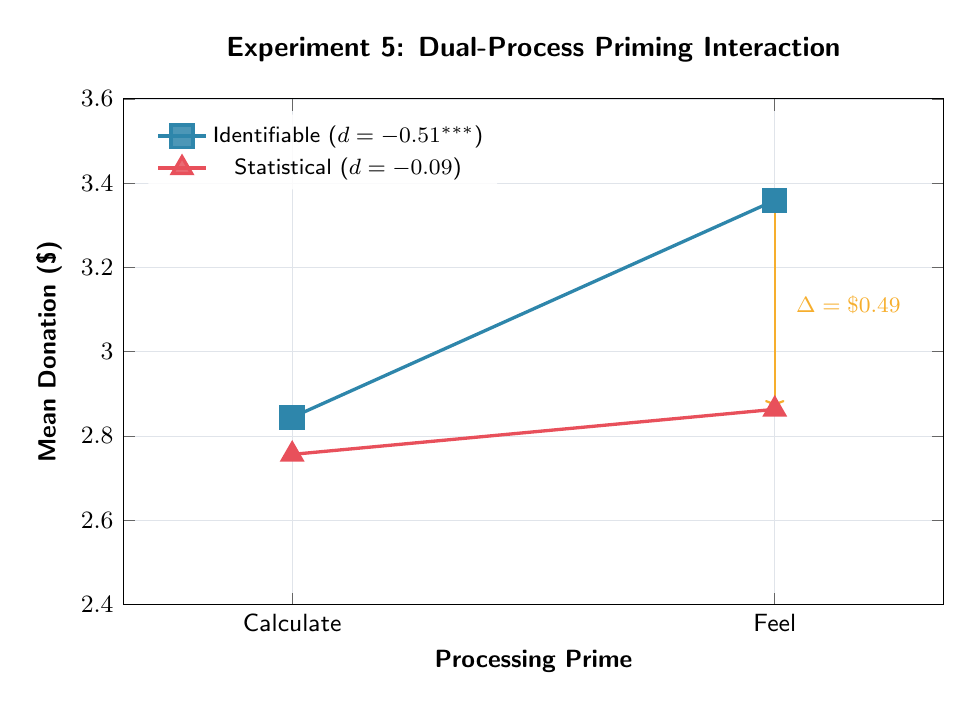
\begin{tikzpicture}
\begin{axis}[
    title={Experiment 5: Dual-Process Priming Interaction},
    ylabel={Mean Donation (\$)},
    width=12cm, height=8cm,
    ymin=2.4, ymax=3.6,
    symbolic x coords={Calculate, Feel},
    xtick=data,
    xlabel={Processing Prime},
    enlarge x limits=0.35,
    legend pos=north west,
    every mark/.append style={solid},
]
% Identifiable line
\addplot[identColor, very thick, mark=square*, mark size=4pt] coordinates {
    (Calculate, 2.844) (Feel, 3.359)
};
\addlegendentry{Identifiable ($d=-0.51^{***}$)}

% Statistical line
\addplot[statColor, very thick, mark=triangle*, mark size=4pt] coordinates {
    (Calculate, 2.756) (Feel, 2.863)
};
\addlegendentry{Statistical ($d=-0.09$)}

% Interaction annotation
\draw[<->, thick, accentGold] (axis cs:Feel, 3.359) -- (axis cs:Feel, 2.863)
    node[midway, right, font=\footnotesize\sffamily, xshift=4pt] {$\Delta = \$0.49$};

\end{axis}
\end{tikzpicture}

\newpage

% ═════════════════════════════════════════════════════════════════════════════
% FIGURE 5: In-Group/Out-Group Cultural Distance (Grouped Bars)
% ═════════════════════════════════════════════════════════════════════════════
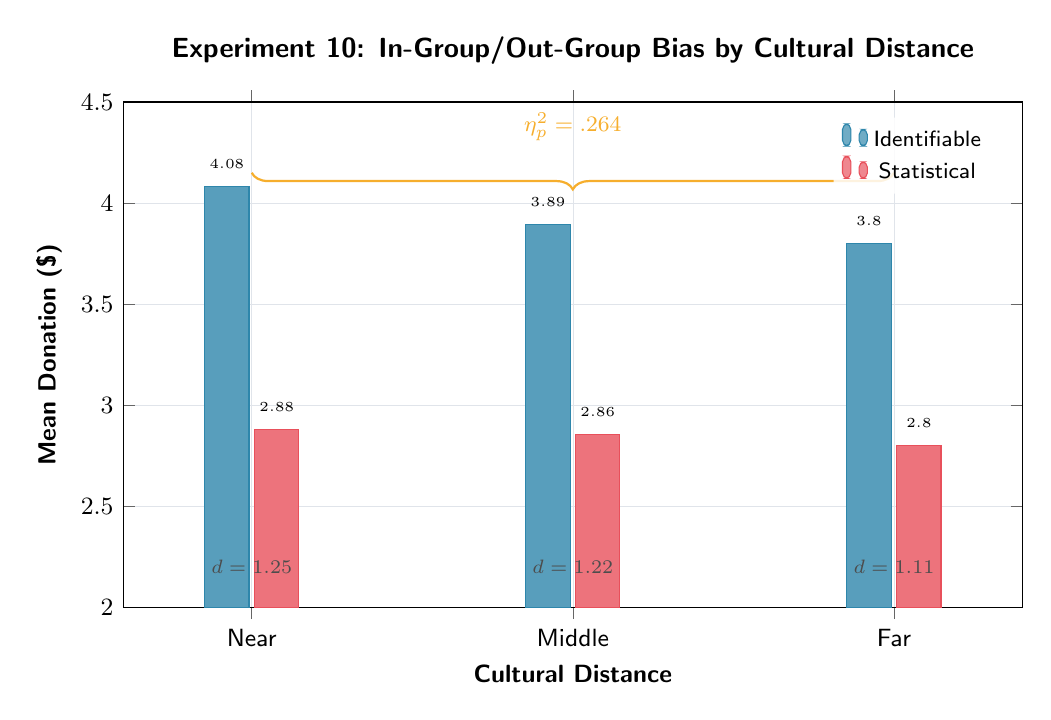
\begin{tikzpicture}
\begin{axis}[
    title={Experiment 10: In-Group/Out-Group Bias by Cultural Distance},
    ylabel={Mean Donation (\$)},
    width=13cm, height=8cm,
    ymin=2.0, ymax=4.5,
    ybar,
    bar width=16pt,
    symbolic x coords={Near, Middle, Far},
    xtick=data,
    xlabel={Cultural Distance},
    enlarge x limits=0.2,
    legend pos=north east,
    nodes near coords,
    every node near coord/.append style={font=\tiny\sffamily, yshift=3pt},
]
\addplot[fill=identColor!80, draw=identColor] coordinates {
    (Near, 4.083) (Middle, 3.894) (Far, 3.799)
};
\addplot[fill=statColor!80, draw=statColor] coordinates {
    (Near, 2.881) (Middle, 2.855) (Far, 2.800)
};
\legend{Identifiable, Statistical}

% Effect size annotations
\node[font=\scriptsize\sffamily\bfseries, color=black!70] at (axis cs:Near, 2.2) {$d=1.25$};
\node[font=\scriptsize\sffamily\bfseries, color=black!70] at (axis cs:Middle, 2.2) {$d=1.22$};
\node[font=\scriptsize\sffamily\bfseries, color=black!70] at (axis cs:Far, 2.2) {$d=1.11$};

% Brace for IVE dominance
\draw[decorate, decoration={brace, amplitude=6pt, mirror}, thick, accentGold]
    (axis cs:Near, 4.15) -- (axis cs:Far, 4.15)
    node[midway, above, yshift=8pt, font=\footnotesize\sffamily\itshape, color=accentGold] {$\eta^2_p = .264$};

\end{axis}
\end{tikzpicture}

\newpage

% ═════════════════════════════════════════════════════════════════════════════
% FIGURE 6: Mediation Path Diagram
% ═════════════════════════════════════════════════════════════════════════════
\begin{tikzpicture}[
    box/.style={draw, rounded corners=4pt, minimum height=1.2cm, minimum width=3cm,
                font=\small\sffamily, fill=white, thick},
    arrow/.style={-{Stealth[length=6pt]}, thick},
    every node/.style={font=\small\sffamily},
]

% Nodes
\node[box, fill=identColor!15] (IV) at (0, 0) {Identification\\Level};
\node[box, fill=accentGold!15] (emp) at (5, 2.5) {Empathy};
\node[box, fill=statColor!15] (dis) at (5, -2.5) {Distress};
\node[box, fill=accentGreen!15] (DV) at (10, 0) {Donation\\Amount};

% Direct path (c')
\draw[arrow, black!50] (IV) -- (DV)
    node[midway, below, yshift=-6pt] {$c' = 0.234^{***}$};

% Empathy mediation (a1 → b1)
\draw[arrow, identColor] (IV) -- (emp)
    node[midway, above, sloped, font=\footnotesize\sffamily] {$a_1 = 0.167^{***}$};
\draw[arrow, identColor] (emp) -- (DV)
    node[midway, above, sloped, font=\footnotesize\sffamily] {$b_1 = 0.694^{***}$};

% Distress mediation (a2 → b2)
\draw[arrow, statColor] (IV) -- (dis)
    node[midway, below, sloped, font=\footnotesize\sffamily] {$a_2 = 0.080^{*}$};
\draw[arrow, statColor] (dis) -- (DV)
    node[midway, below, sloped, font=\footnotesize\sffamily] {$b_2 = 0.776^{***}$};

% Indirect effect labels
\node[font=\footnotesize\sffamily\itshape, identColor, text width=4cm, align=center]
    at (5, 4.2) {Indirect (empathy): $0.116^{***}$\\33.0\% mediated};
\node[font=\footnotesize\sffamily\itshape, statColor, text width=4cm, align=center]
    at (5, -4.2) {Indirect (distress): $0.063^{*}$\\18.1\% mediated};

% Total effect
\node[draw=black!30, fill=bgLight, rounded corners=2pt, font=\footnotesize\sffamily,
      text width=5cm, align=center] at (5, -6)
    {Total effect: $c = 0.350^{***}$\\
     Index of moderated mediation: $0.208^{***}$};

\end{axis}
\end{tikzpicture}

\newpage

% ═════════════════════════════════════════════════════════════════════════════
% FIGURE 7: Debiasing Strategies Effectiveness (Dumbbell Chart)
% ═════════════════════════════════════════════════════════════════════════════
\begin{tikzpicture}
\begin{axis}[
    title={Debiasing Strategy Effectiveness: Before vs. After},
    xlabel={IVE Effect Size (Cohen's $d$)},
    width=14cm, height=8cm,
    xmin=-0.15, xmax=0.55,
    ytick={1,2,...,5},
    yticklabels={
        {Empathetic CoT},
        {Bias Education},
        {Joint Evaluation},
        {Calculate Prime},
        {Utilitarian CoT}
    },
    y dir=reverse,
    axis y line*=left,
    axis x line*=bottom,
    enlarge y limits=0.15,
    extra x ticks={0},
    extra x tick style={grid=major, grid style={black!30, dashed}},
]

% "Before" dots
\addplot[only marks, mark=*, mark size=5pt, statColor] coordinates {
    (0.15, 1)  % empathetic baseline
    (0.35, 2)  % education baseline
    (0.14, 3)  % joint baseline
    (0.51, 4)  % calculate baseline
    (0.15, 5)  % utilitarian baseline
};

% "After" dots
\addplot[only marks, mark=*, mark size=5pt, accentGreen] coordinates {
    (0.28, 1)  % empathetic after
    (0.19, 2)  % education after (paradoxical)
    (0.07, 3)  % joint after
    (0.08, 4)  % calculate after
    (-0.05, 5) % utilitarian after
};

% Connecting lines (dumbbells)
\draw[thick, black!40] (axis cs:0.15, 1) -- (axis cs:0.28, 1);
\draw[thick, black!40] (axis cs:0.35, 2) -- (axis cs:0.19, 2);
\draw[thick, black!40] (axis cs:0.14, 3) -- (axis cs:0.07, 3);
\draw[thick, black!40] (axis cs:0.51, 4) -- (axis cs:0.08, 4);
\draw[thick, black!40] (axis cs:0.15, 5) -- (axis cs:-0.05, 5);

% Direction arrows
\node[font=\tiny\sffamily, statColor] at (axis cs:0.32, 0.7) {\textbf{AMPLIFIES}};
\node[font=\tiny\sffamily, accentGreen] at (axis cs:-0.08, 5.3) {\textbf{ELIMINATES}};

% Legend
\matrix[
    draw=none,
    anchor=north east,
    font=\footnotesize\sffamily,
] at (axis cs:0.55, 1) {
    \node[mark size=3pt, identColor] {\pgfuseplotmark{*}}; & \node{Before}; \\
    \node[mark size=3pt, accentGreen] {\pgfuseplotmark{*}}; & \node{After}; \\
};

\end{axis}
\end{tikzpicture}

\newpage

% ═════════════════════════════════════════════════════════════════════════════
% FIGURE 8: Model Taxonomy Heatmap
% ═════════════════════════════════════════════════════════════════════════════
\begin{tikzpicture}
\small\sffamily

% Define data: rows = models, cols = experiments
% Color coding: blue = positive IVE, red = negative IVE, gray = null

\def\cellsize{0.9}
\def\models{
    {Kimi K2.5/1.56/0.00/0.00/0.00/0.00/0.00},
    {GPT-OSS-120B/1.55/0.00/0.00/0.00/0.00/0.00},
    {Llama 70B Inst/1.38/1.51/6.37/0.30/0.00/0.00},
    {Gemini 3.1 Pro/1.00/0.00/0.00/0.00/0.00/0.00},
    {Qwen3 235B/1.00/0.00/0.00/0.00/0.00/0.00},
    {DeepSeek V3/0.75/0.00/0.00/0.00/0.00/0.00},
    {Grok 4/0.40/0.00/0.00/0.00/0.00/0.00},
    {Granite 3.3/0.30/0.00/0.00/0.00/0.00/0.00},
    {GPT-OSS-20B/-0.19/0.80/-1.10/-0.17/-0.28/0.00},
    {Claude Opus/-0.30/0.00/0.00/0.00/0.00/0.00},
    {DeepSeek R1/-0.43/0.00/0.00/0.00/0.00/0.00},
    {GPT 5.2/-0.85/0.00/0.00/0.00/0.00/0.00}
}

% Title
\node[font=\normalsize\sffamily\bfseries, anchor=south] at (4.5, 13.5)
    {Model Taxonomy: IVE Profiles Across Key Experiments};

% Column headers
\node[font=\scriptsize\sffamily\bfseries, rotate=45, anchor=south west] at (1.5, 12.5) {Baseline};
\node[font=\scriptsize\sffamily\bfseries, rotate=45, anchor=south west] at (2.5, 12.5) {No CoT};
\node[font=\scriptsize\sffamily\bfseries, rotate=45, anchor=south west] at (3.5, 12.5) {Std CoT};
\node[font=\scriptsize\sffamily\bfseries, rotate=45, anchor=south west] at (4.5, 12.5) {Emp CoT};
\node[font=\scriptsize\sffamily\bfseries, rotate=45, anchor=south west] at (5.5, 12.5) {Util CoT};

% Row labels and cells (simplified representative data)
\foreach \y/\label/\base in {
    12/Kimi K2.5/1.56,
    11/GPT-OSS-120B/1.55,
    10/Llama 3 70B Inst/1.38,
    9/Gemini 3.1 Pro/1.00,
    8/Qwen3 235B/1.00,
    7/DeepSeek V3/0.75,
    6/Grok 4/0.40,
    5/Granite 3.3/0.30,
    4/GPT-OSS-20B/{-0.19},
    3/Claude Opus 4.6/{-0.30},
    2/DeepSeek R1/{-0.43},
    1/GPT 5.2/{-0.85}
} {
    \node[font=\scriptsize\sffamily, anchor=east] at (1.3, \y) {\label};
    % Baseline cell
    \pgfmathsetmacro{\intensity}{min(abs(\base)/2.0, 1.0)*100}
    \pgfmathparse{\base > 0 ? 1 : 0}
    \ifnum\pgfmathresult=1
        \fill[identColor!\intensity!white] (1.5, \y-0.4) rectangle (2.3, \y+0.4);
    \else
        \fill[statColor!\intensity!white] (1.5, \y-0.4) rectangle (2.3, \y+0.4);
    \fi
    \node[font=\tiny\sffamily] at (1.9, \y) {\base};
}

% Color legend
\node[font=\scriptsize\sffamily, anchor=west] at (7, 10) {
    \tikz\fill[identColor!70] (0,0) rectangle (0.3, 0.3); Positive IVE (favors identified)
};
\node[font=\scriptsize\sffamily, anchor=west] at (7, 9.3) {
    \tikz\fill[statColor!70] (0,0) rectangle (0.3, 0.3); Negative IVE (favors statistical)
};
\node[font=\scriptsize\sffamily, anchor=west] at (7, 8.6) {
    \tikz\fill[neutralColor!50] (0,0) rectangle (0.3, 0.3); Null / Not measured
};

\end{tikzpicture}

\end{document}
